\documentclass[aspectratio=169,11pt]{beamer}

% ============================================================
% SISMID 2026 -- Day 1, 9:45 session
% Agent Coding Introduction (S. Yang + C. Djorno)
% Setup -> AI coding agents -> first data scrape
% Compile: pdflatex agent-coding-intro.tex  (run twice)
% ============================================================

\IfFileExists{beamerthememetropolis.sty}{
  \usetheme{metropolis}
  \metroset{progressbar=frametitle, sectionpage=progressbar, numbering=fraction}
}{
  \usetheme{Boadilla}
  \usecolortheme{seahorse}
  \setbeamertemplate{navigation symbols}{}
}

\usepackage[utf8]{inputenc}
\usepackage[T1]{fontenc}
\usepackage{tikz}
\usetikzlibrary{arrows.meta, positioning, fit, backgrounds, calc}
\usepackage{xcolor}
\usepackage{listings}

\definecolor{AccentA}{HTML}{2A6F97}
\definecolor{AccentB}{HTML}{C1666B}
\definecolor{AccentC}{HTML}{3B8A5B}
\setbeamercolor{frametitle}{bg=AccentA}
\setbeamercolor{progress bar}{fg=AccentB}

\definecolor{skbg}{rgb}{0.96,0.96,0.94}
\lstdefinestyle{prompt}{
  basicstyle=\ttfamily\scriptsize,
  backgroundcolor=\color{skbg},
  showstringspaces=false, breaklines=true,
  frame=single, framesep=4pt, columns=fullflexible, numbers=none,
}
\lstset{style=prompt}

\tikzset{
  cbox/.style={draw=AccentA, very thick, rounded corners, align=center,
    minimum height=1.0cm, inner sep=6pt, font=\small, fill=AccentA!6},
  sbox/.style={draw=AccentA, thick, rounded corners, align=center,
    minimum height=0.85cm, inner sep=4pt, font=\scriptsize, fill=AccentA!6},
  rbox/.style={draw=AccentB, thick, rounded corners, align=center,
    minimum height=0.85cm, inner sep=4pt, font=\scriptsize, fill=AccentB!8},
  gbox/.style={draw=AccentC, thick, rounded corners, align=center,
    minimum height=0.85cm, inner sep=4pt, font=\scriptsize, fill=AccentC!8},
  flow/.style={-{Stealth[length=3mm]}, very thick, draw=AccentB},
  flowq/.style={-{Stealth[length=2.4mm]}, thick, draw=AccentA!70},
}

\title{Agent Coding Introduction}
\subtitle{Set up the environment, stand up an agent, take your first scrape}
\author{Shihao Yang \quad\textbullet\quad Candice Djorno}
\institute{SISMID 2026 \textbullet\ Day 1, 9:45}
\date{July 20, 2026}

\begin{document}

\begin{frame}
  \titlepage
\end{frame}

\begin{frame}{What this first hour is for}
  Mauricio just gave you the big picture. Now we get your hands on a keyboard.

  \medskip
  By the end of this session everyone in the room will have:
  \begin{enumerate}
    \item an \textbf{identical coding environment}, with nothing installed locally,
    \item a working \textbf{AI coding agent} (Codex, Claude Code, or Antigravity CLI) you set up yourself,
    \item and your \textbf{first scraped data stream}: real numbers pulled from the
          open web, plotted and sanity-checked.
  \end{enumerate}
  \vfill
  \begin{alertblock}{The promise}
    You will not write a data-collection platform. You will describe what you want,
    the agent (or a pre-filled notebook) fetches it, and you keep the judgment.
  \end{alertblock}
\end{frame}

% ---------------------------------------------------------------
\section{One environment for everyone}

\begin{frame}{The room we are teaching}
  \begin{columns}[T]
    \begin{column}{0.48\textwidth}
      \textbf{Keep it streamlined}
      \begin{itemize}
        \item one bad install can cost an hour
        \item wants a result to keep
      \end{itemize}
    \end{column}
    \begin{column}{0.48\textwidth}
      \textbf{Lightweight and ready for non-coder}
      \begin{itemize}
        \item done in five minutes
        \item wants the real data plumbing
      \end{itemize}
    \end{column}
  \end{columns}
  \vfill
  \begin{block}{Two moves serve both}
    An \textbf{identical environment} removes the setup lottery. An \textbf{agent}
    lifts the novice to a working result and frees the expert from boilerplate. The
    agent is the equalizer we lean on all week.
  \end{block}
\end{frame}

\begin{frame}{Pick a lane to get the environment}
  Same repository, three ways in. Codespaces is the supported path.
  \begin{itemize}
    \item \textbf{GitHub Codespace (recommended).} A preconfigured container in your
          browser. Nothing to install. Free on your own account.
    \item \textbf{Clone and run locally.} If you prefer your own machine:
          \texttt{pip install -r requirements.txt} on Python 3.12.
    \item \textbf{Google Colab.} Open the notebooks with just a Google account.
  \end{itemize}
  \vspace{0.4em}
  \begin{exampleblock}{Launch a Codespace (do this now)}
    \texttt{github.com/Shihao-Yang/sismid2026} $\rightarrow$ green \texttt{Code}
    button $\rightarrow$ \texttt{Codespaces} $\rightarrow$
    \texttt{Create codespace on main}. Builds in about a minute.
  \end{exampleblock}
\end{frame}

\begin{frame}{Confirm it works: the smoke test}
  Before anything else, prove the environment is healthy.
  \begin{itemize}
    \item Open \texttt{notebooks/00\_smoke\_test.ipynb} and run all cells, or in a
          terminal run \texttt{python scripts/smoke\_test.py}.
    \item You should see library versions and \textbf{``Environment OK''}.
  \end{itemize}
  \vspace{0.5em}
  \begin{center}
    \itshape If the smoke test passes, the rest of the week has no ``it works on my
    laptop'' problem. That is the whole point of a shared container.
  \end{center}
\end{frame}

% ---------------------------------------------------------------
\section{Standing up a coding agent}

\begin{frame}{What is a coding agent?}
  A coding agent is an LLM that can \textbf{read your files, run code, see the error,
  and try again}, inside your project, from a plain-English request.

  \medskip
  \begin{columns}[T]
    \begin{column}{0.32\textwidth}
      \textbf{OpenAI Codex}
      \begin{itemize}
        \item CLI, runs in the Codespace terminal
      \end{itemize}
    \end{column}
    \begin{column}{0.32\textwidth}
      \textbf{Claude Code}
      \begin{itemize}
        \item CLI, runs in the Codespace terminal
      \end{itemize}
    \end{column}
    \begin{column}{0.32\textwidth}
      \textbf{Antigravity CLI}
      \begin{itemize}
        \item CLI (\texttt{agy}), free Google login
      \end{itemize}
    \end{column}
  \end{columns}
  \medskip
  All three are command-line agents: one script installs them and they run right in the
  browser Codespace. We set up all three so you can compare them on the same task.
  \vfill
  \begin{center}
    \itshape Not autocomplete. A junior collaborator that does the typing and the
    debugging while you keep the judgment.
  \end{center}
\end{frame}

\begin{frame}[fragile]{Install and authenticate (together, in class)}
  The container ships \emph{no} agent on purpose, so you learn to do this yourself.
  \begin{lstlisting}
# 1. install all three CLIs
bash scripts/setup-agents.sh

# 2. log in (class passcode announced in class)
bash   scripts/codex-login.sh    # Codex
source scripts/claude-login.sh   # Claude Code
agy                              # Antigravity: your own Google login
  \end{lstlisting}
  \begin{itemize}
    \item \texttt{source} for Claude (it exports a token into \emph{this} shell);
          \texttt{bash} for Codex (it just writes \texttt{\textasciitilde{}/.codex/auth.json}).
    \item You are identified by your GitHub username, so a Codespace restart hands you
          back the \emph{same} credential.
    \item \textbf{Golden rule:} keys never get committed and never get pasted into a
          notebook cell.
    \item Sanity check: ``list the CSV files in \texttt{data/} and print the first rows
          of each.''
  \end{itemize}
\end{frame}

\begin{frame}{Two lanes, one destination}
  \begin{center}
  \resizebox{0.74\textwidth}{!}{%
  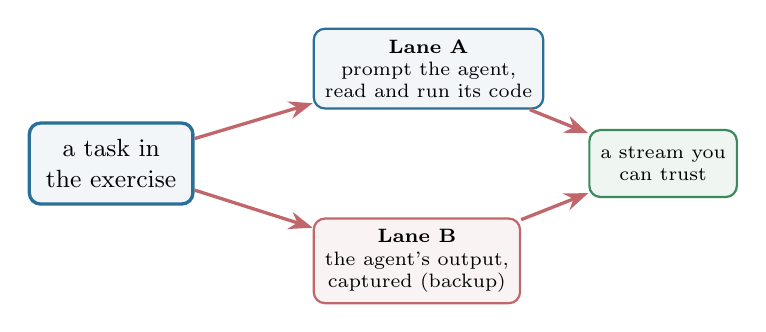
\begin{tikzpicture}[node distance=0.55cm and 1.4cm]
    \node[cbox] (goal) {a task in\\the exercise};
    \node[sbox, above right=0.15cm and 1.5cm of goal] (a) {\textbf{Lane A}\\prompt the agent,\\read and run its code};
    \node[rbox, below right=0.15cm and 1.5cm of goal] (b) {\textbf{Lane B}\\the agent's output,\\captured (backup)};
    \node[gbox, right=5.0cm of goal] (out) {a stream you\\can trust};
    \draw[flow] (goal) -- (a);
    \draw[flow] (goal) -- (b);
    \draw[flow] (a) -- (out);
    \draw[flow] (b) -- (out);
  \end{tikzpicture}}
  \end{center}
  \begin{itemize}
    \item Agent not authenticated yet? Use Lane B and come back. Nobody is blocked.
    \item New to this? Pair with a neighbor: an expert partner plus the agent is the
          fastest way to learn what good output looks like.
    \item TA and instructors circulate. Raise a hand early, not after an hour.
  \end{itemize}
\end{frame}

% ---------------------------------------------------------------
\section{Your first scrape}

\begin{frame}{Let's build one, live}
  ``Scraping'' just means fetching web data into a table you can model. We are going to
  do it \textbf{right now}, together, and you follow along.
  \vspace{0.3em}
  \begin{block}{The goal on screen in the next five minutes}
    Dengue search interest for \textbf{Mexico}, the \textbf{past 5 years}, as a tidy,
    reproducible CSV that ends on \emph{this week}. Plus the historical 2004-2011 window
    that feeds the 11:00 model.
  \end{block}
  \vspace{0.3em}
  We do it two ways: first by hand on the website, then by handing one prompt to an
  agent. Watch the difference.
\end{frame}

\begin{frame}{The old way: open the website}
  \begin{exampleblock}{Open}
    \texttt{trends.google.com} $\;\rightarrow\;$ search \textbf{dengue}
    $\;\rightarrow\;$ region \textbf{Mexico} $\;\rightarrow\;$ past \textbf{5 years}.
  \end{exampleblock}
  \medskip
  You get a clean 0-100 curve you can eyeball. But for real work it fights you:
  \begin{itemize}
    \item values \textbf{rescale} the moment you add or drop a term,
    \item you can compare at most \textbf{5 terms} at once,
    \item getting it into code, \textbf{reproducibly}, means clicking export every time.
  \end{itemize}
  \vspace{0.2em}
  \begin{center}
    \itshape Fine for a look, hopeless as a pipeline. So let's have an agent script
    exactly this, dengue being the backbone signal we model at 11:00.
  \end{center}
\end{frame}

\begin{frame}{The loop that every stream will use}
  \begin{center}
  \resizebox{0.97\textwidth}{!}{%
  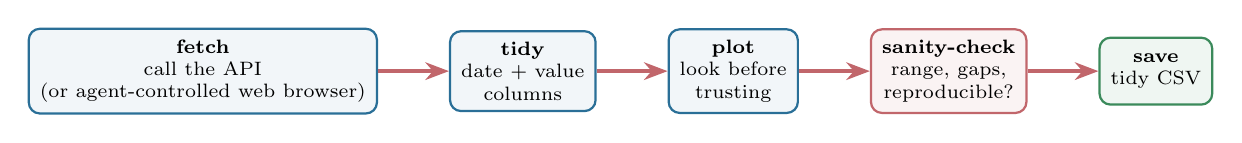
\begin{tikzpicture}[node distance=0.9cm]
    \node[sbox] (f) {\textbf{fetch}\\call the API \\ (or agent-controlled web browser)};
    \node[sbox, right=of f] (t) {\textbf{tidy}\\date + value\\columns};
    \node[sbox, right=of t] (p) {\textbf{plot}\\look before\\trusting};
    \node[rbox, right=of p] (s) {\textbf{sanity-check}\\range, gaps,\\reproducible?};
    \node[gbox, right=of s] (v) {\textbf{save}\\tidy CSV};
    \draw[flow] (f) -- (t);
    \draw[flow] (t) -- (p);
    \draw[flow] (p) -- (s);
    \draw[flow] (s) -- (v);
  \end{tikzpicture}}
  \end{center}
  \vspace{0.5em}
  \begin{center}
    \itshape Learn it once here. Google Trends, wastewater, mobility, and news all reuse
    the exact same five steps.
  \end{center}
\end{frame}

\begin{frame}{Now let an agent do it}
  Same goal, handed to an agent instead of your mouse. Pick one and open it:
  \begin{exampleblock}{Open (pick one)}
    \begin{itemize}
      \item \textbf{Codex}: type \texttt{codex} in the Codespace terminal
      \item \textbf{Claude Code}: type \texttt{claude} in the Codespace terminal
      \item \textbf{Antigravity CLI}: type \texttt{agy} in the Codespace terminal
    \end{itemize}
  \end{exampleblock}
  \begin{center}
    \itshape All three take the same plain-English goal and run in the same terminal.
    Pick whichever you like.
  \end{center}
\end{frame}

\begin{frame}[fragile]{Give it one prompt}
  \begin{block}{Prompt (paste this)}
  \begin{lstlisting}
Pull Google Trends for a handful of dengue
terms in Mexico: "dengue", "sintomas de dengue",
"mosquito", over the past 5 years. Return a
tidy date + one-column-per-term DataFrame. Plot the three series
and print the date of the last point.
  \end{lstlisting}
  \end{block}
  \begin{center}
    \itshape One paragraph. No API keys, no boilerplate. This is the whole live flow.
  \end{center}
\end{frame}

\begin{frame}{What comes back}
  The agent writes \texttt{gt\_fetch(...)}, runs it, and hands you:
  \begin{exampleblock}{Result (a real run, July 2026)}
    262 weekly points $\times$ 3 terms, Jul 2021 to \textbf{the week of Jul 12--18, 2026}.
    The last point is \emph{this week}: the pull is genuinely live.
  \end{exampleblock}
  \begin{itemize}
    \item A plot of the three dengue terms appears, current through today.
    \item The exact code it wrote is captured in the \textbf{Lane B} notebook, so a
          rate-limited neighbor sees the same thing.
  \end{itemize}
  \vspace{0.1em}
  \begin{center}
    \itshape From a sentence to a live, reproducible signal. That is the point.
  \end{center}
\end{frame}

\begin{frame}{Verify what came back (your job, not the agent's)}
  Every scraped stream earns a few cheap checks before it enters a model:
  \begin{itemize}
    \item \textbf{Range and gaps:} does the date span match what you asked? Missing
          months quietly become wrong models.
    \item \textbf{Scale sanity:} plausible values, not all zeros or a flat line from a
          failed pull.
    \item \textbf{Reproducibility:} pull twice. Because Google samples searches, repeat
          pulls can \emph{differ} (a little on the public 0-100 endpoint, a lot on the raw
          Health Trends API). That is what this afternoon's preprocessing fixes.
    \item \textbf{Face validity:} do the peaks land in a plausible Mexican dengue season?
  \end{itemize}
  \vspace{0.3em}
  \begin{alertblock}{The habit to build}
    One plot and one sanity question per stream. This is the skill, more than the fetch.
  \end{alertblock}
\end{frame}

\begin{frame}{When Google Trends fights back (it will)}
  A live pull often hits a \textbf{429 (too many requests)}, then succeeds on the next
  try. That is normal. Two things keep you moving:
  \begin{itemize}
    \item \textbf{Retry.} The notebook waits and retries automatically. We tested this from
          a Codespace on an \textbf{Azure} datacenter IP: 429, wait, then success. Usually
          enough.
    \item \textbf{The cache (Lane B).} If it still will not budge, the notebook falls back
          to the cached CSV, so you are never stuck.
  \end{itemize}
  \vspace{0.3em}
  \begin{center}
    \itshape If a block is ever really stubborn, there is a proper fix: routing through a
    proxy or VPN. We cover that this afternoon, in the data-scraping session.
  \end{center}
\end{frame}

\begin{frame}{Now you: Exercise 0}
  Open \texttt{exercise/exercise0\_data\_scraping} and work either lane.
  \begin{itemize}
    \item Set up the environment and pass the smoke test.
    \item Stand up an agent (or use Lane B).
    \item Scrape dengue search interest for Mexico, add related terms, sanity-check, save
          a tidy CSV.
    \item Discuss: why might search interest rise without any real change in disease
          activity, and what do you do about two pulls disagreeing?
  \end{itemize}
  \vspace{0.4em}
  \begin{block}{What to walk away with}
    The dengue search CSV you scraped yourself (ready for 11:00), and the
    fetch-tidy-plot-check-save reflex. Swap in your own country and disease if you finish
    early.
  \end{block}
\end{frame}

\begin{frame}{Looking ahead}
  \begin{itemize}
    \item \textbf{Next (11:00):} the Dengue exercise. Intro to Google Dengue Trends, then
          map the search series you just scraped onto dengue cases with least squares.
    \item \textbf{This afternoon:} Google Trends in depth, where the same scrape returns
          different numbers each time and needs statistical preprocessing.
    \item \textbf{All week:} the agent stays your coding tool, and Lane B is always there.
  \end{itemize}
  \vfill
  \begin{center}
    \itshape You now have an environment, an agent, and a scraped dengue signal. That is
    the entire foundation the rest of the course builds on.
  \end{center}
\end{frame}

\begin{frame}[standout]
  Questions?\\[0.4em]
  \small Repo: \texttt{github.com/Shihao-Yang/sismid2026}
\end{frame}

\end{document}
